\documentclass[11pt]{article}
\usepackage[margin=1in]{geometry}
\usepackage{booktabs}
\usepackage{amsmath}
\usepackage{hyperref}
\usepackage[T1]{fontenc}
\usepackage[utf8]{inputenc}
\usepackage{graphicx}
\usepackage{float}
\usepackage{setspace}
\onehalfspacing

\graphicspath{{../results/figures/}}

\title{Supplementary Methods\\Dispersion, not displacement: loss of alveolar epithelial state coherence in lethal COVID-19}
\author{}
\date{}

\begin{document}
\maketitle

\section{Donor-level inference}

\subsection{Donor summary statistics}

For each of the 27 donors, we computed the following cell-level summary statistics by aggregating across all alveolar epithelial cells from that donor:
\begin{itemize}
    \item \textbf{Median pseudotime}: median diffusion pseudotime across all cells from the donor.
    \item \textbf{IQR pseudotime}: interquartile range of pseudotime.
    \item \textbf{Within-donor dispersion}: variance of Euclidean distances from each cell to the donor's centroid in 50-dimensional PCA space.
    \item \textbf{Median distance to donor centroid}: median Euclidean distance from cells to the donor's PCA centroid.
    \item \textbf{Fraction transitional}: fraction of cells annotated as ECM-high epithelial.
    \item \textbf{Program scores}: median score for each of 8 gene programs.
\end{itemize}

\subsection{Donor-level statistical tests}

All primary comparisons use the donor (not the cell) as the inferential unit. For each metric, we performed a two-sided Mann--Whitney $U$ test comparing COVID-19 donors ($n = 20$) against healthy donors ($n = 7$). Effect sizes are reported as rank-biserial correlations: $r = 1 - 2U/(n_1 n_2)$.

\subsection{Bootstrap confidence intervals}

We computed 10,000-replicate bootstrap confidence intervals for the difference in donor-level medians between conditions. At each replicate, we resampled donors (not cells) with replacement within each condition group and computed the difference in group medians. The 95\% CI was taken as the 2.5th and 97.5th percentiles of the bootstrap distribution.

\textbf{Results:}
\begin{itemize}
    \item Pseudotime: observed difference $+0.041$, 95\% CI $[-0.013, 0.086]$
    \item Within-donor dispersion: observed difference $+6.84$, 95\% CI $[-30.7, 16.5]$
    \item Fraction transitional: observed difference $+0.009$, 95\% CI $[-0.053, 0.020]$
\end{itemize}

The bootstrap CI for pseudotime marginally includes zero, reflecting the low power of a 7-versus-20 comparison. The cell-level permutation test ($p = 0.001$) and cross-cohort replication ($p = 0.002$ at donor level) provide independent corroboration.

\subsection{OLS donor-level model}

We fit an ordinary least-squares regression: $\text{median\_pseudotime} \sim \text{is\_covid}$, treating each donor as one observation ($n = 27$). A random intercept for donor is unnecessary at this level because each donor contributes exactly one observation.

\textbf{Results:} COVID-19 coefficient $= +0.043$ (95\% CI $[0.010, 0.076]$; $p = 0.013$; $R^2 = 0.22$).

\subsection{Donor-level dispersion comparison}

For each donor, we computed the median Euclidean distance from the donor's cells to the donor's centroid in PCA space. We then compared per-donor median dispersions between conditions using a one-sided Mann--Whitney $U$ test (alternative: COVID $>$ Healthy) and Levene's test on the per-donor dispersion values.

\textbf{Results:} COVID-19 donors had median per-donor dispersion $= 7.77$; healthy donors had $= 10.58$ (Mann--Whitney $p = 0.999$; Levene $p = 0.071$). This indicates that the cell-level dispersion finding (Levene $p < 10^{-30}$) arises from between-donor heterogeneity within the COVID-19 condition, not from uniform within-donor inflation.

\section{Portable state scores}

Six continuous state scores were computed for each cell:

\begin{enumerate}
    \item \textbf{AT2 identity}: mean expression of AT2 markers (SFTPC, SFTPA1, SFTPA2, ABCA3, LAMP3, SLC34A2, NAPSA, PGC, LPCAT1).
    \item \textbf{AT1 identity}: mean expression of AT1 markers (AGER, PDPN, HOPX, CLIC5, CAV1, EMP2, AKAP5, RTKN2).
    \item \textbf{Transitional}: mean expression of transitional markers (KRT8, CLDN4, SFN, KRT18, LGALS3, HOPX, AGER, PDPN) from the AT2-to-AT1 differentiation program.
    \item \textbf{Injury composite}: mean of per-cell scores for the six non-homeostatic programs (interferon, NF-$\kappa$B, oxidative stress, apoptosis, senescence, AT2-to-AT1 differentiation).
    \item \textbf{Coherence loss}: Euclidean distance from each cell to the centroid of healthy cells in PCA space.
    \item \textbf{Repair failure}: transitional score $- 0.5 \times$ (AT2 identity $+$ AT1 identity).
\end{enumerate}

\subsection{Benchmark results (primary atlas)}

\begin{table}[h]
\centering
\small
\begin{tabular}{lrrrrr}
\toprule
Score & $\rho$(pseudotime) & MW $p$ (condition) & COVID median & Healthy median & AUC (transitional) \\
\midrule
AT2 identity & $-0.693$ & $1.7 \times 10^{-25}$ & 0.650 & 0.605 & 0.323 \\
AT1 identity & $+0.687$ & $5.7 \times 10^{-5}$ & 0.394 & 0.348 & 0.375 \\
Transitional & $+0.282$ & $1.3 \times 10^{-20}$ & 0.285 & 0.278 & 0.441 \\
Injury composite & $+0.276$ & $3.8 \times 10^{-70}$ & $-0.007$ & $-0.024$ & 0.630 \\
Coherence loss & $+0.412$ & $1.1 \times 10^{-72}$ & 10.68 & 11.56 & 0.972 \\
Repair failure & $+0.265$ & $1.3 \times 10^{-55}$ & $-0.342$ & $-0.407$ & 0.730 \\
\bottomrule
\end{tabular}
\caption{State score benchmarks on primary atlas. $\rho$: Spearman correlation with pseudotime. MW: Mann--Whitney $U$ test between conditions. AUC: area under ROC curve for detecting annotated transitional cells.}
\end{table}

The coherence-loss score achieves AUC $= 0.972$ for transitional-cell detection, confirming that geometry-based scores capture the transitional phenotype without requiring marker thresholds.

\subsection{Replication cohort state scores}

All six state scores were computed on the independent replication cohort (89,736 cells, 618 donors) using available genes from the 84-gene panel. PCA was recomputed on the replication data. All scores showed significant condition separation ($p < 10^{-300}$), confirming that the continuous, manifold-based scoring approach transfers across cohorts where marker-threshold DATP calling fails.

\section{Program-geometry linkage}

For each of 8 gene programs, we computed:
\begin{enumerate}
    \item Spearman $\rho$ with Euclidean distance to healthy centroid in PCA space.
    \item Spearman $\rho$ with diffusion pseudotime.
\end{enumerate}

AT2 identity was most strongly anti-correlated with both distance ($\rho = -0.18$) and pseudotime ($\rho = -0.70$). AT2-to-AT1 differentiation was the strongest positive correlate of pseudotime ($\rho = 0.31$) and distance ($\rho = 0.17$).

\subsection{Fan-out contribution}

We decomposed the fan-out by regressing distance-to-healthy-centroid on all 8 program scores (linear regression, $R^2 = 0.115$). Top contributors: senescence (coefficient $= 6.83$), oxidative stress ($3.83$), NF-$\kappa$B ($1.95$). Negative contributors: AT2 identity ($-1.13$), AT1 identity ($-1.02$). This indicates that the dispersion pattern is driven by divergent activation of stress/senescence programs across cells.

\subsection{Repair-stall analysis}

We computed the ratio of AT2-to-AT1 differentiation score to apoptosis score in 10 equal-width pseudotime bins, stratified by condition. In healthy controls, the differentiation/apoptosis ratio was consistently higher than in COVID-19 at late pseudotime, consistent with a model where COVID-19 cells initiate repair but are diverted toward apoptotic rather than differentiation endpoints.

\section{Software}

All analyses were performed in Python 3.12.3 using: Scanpy 1.12.1, AnnData 0.12.10, NumPy 2.4.3, SciPy 1.17.1, pandas 2.3.3, statsmodels 0.14.6, scikit-learn 1.8.0. Random seeds fixed to 42 throughout.

\clearpage
\section{Supplementary Figures}

\begin{figure}[H]
\centering
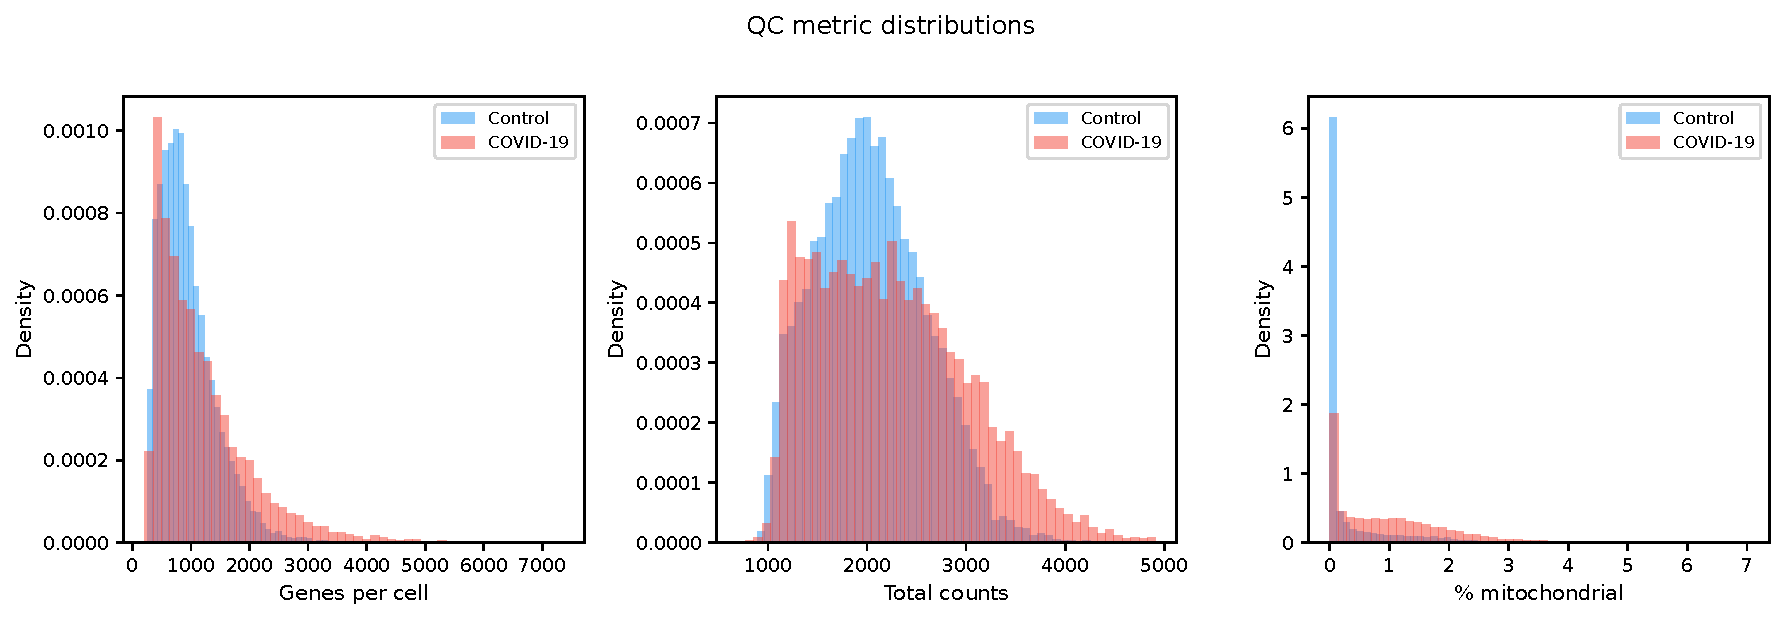
\includegraphics[width=\textwidth]{figS1_qc.pdf}
\caption{\textbf{Figure S1: Quality control.} Per-donor cell counts, gene counts, and mitochondrial fraction distributions for the 22,128 alveolar epithelial cells across 27 donors.}
\label{fig:S1}
\end{figure}

\begin{figure}[H]
\centering
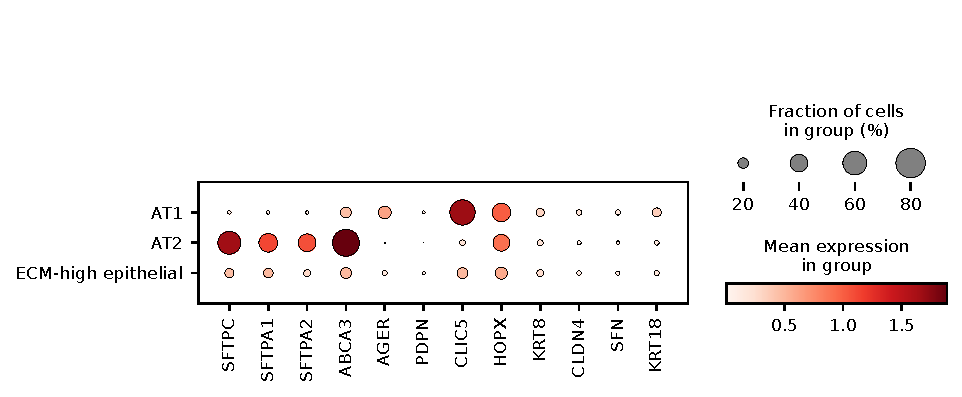
\includegraphics[width=\textwidth]{figS2_markers.pdf}
\caption{\textbf{Figure S2: Marker gene expression.} Expression of canonical AT1 (AGER, HOPX), AT2 (SFTPC, SFTPA1), and transitional (KRT8, CLDN4) markers across annotated cell types, confirming annotation quality.}
\label{fig:S2}
\end{figure}

\begin{figure}[H]
\centering
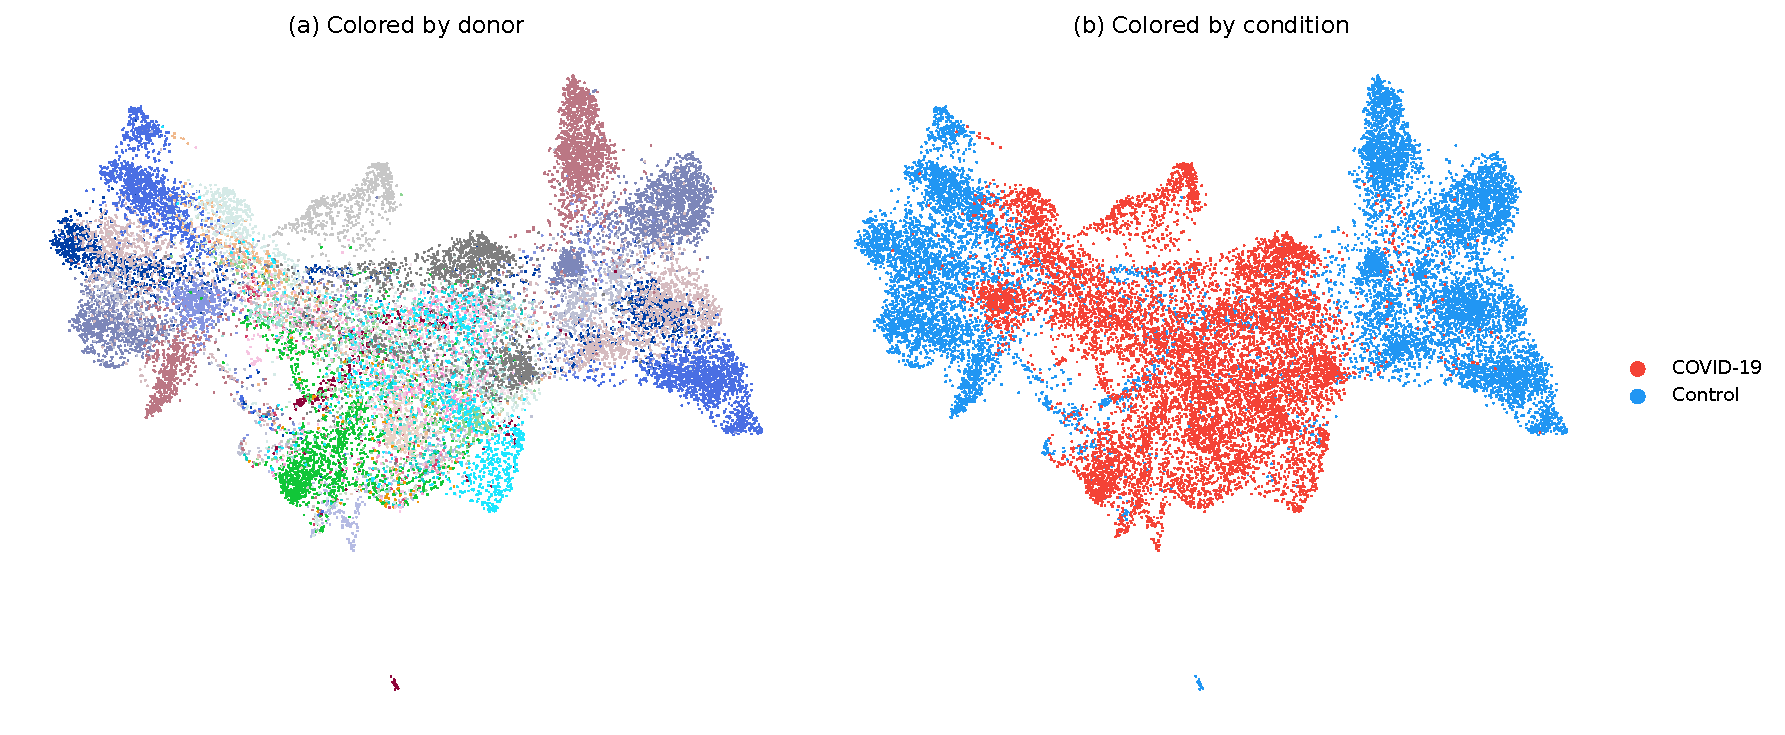
\includegraphics[width=\textwidth]{figS3_batch.pdf}
\caption{\textbf{Figure S3: Batch structure.} UMAP colored by donor ID and Harmony-corrected embedding, showing batch correction convergence and its effect on pseudotime estimation.}
\label{fig:S3}
\end{figure}

\begin{figure}[H]
\centering
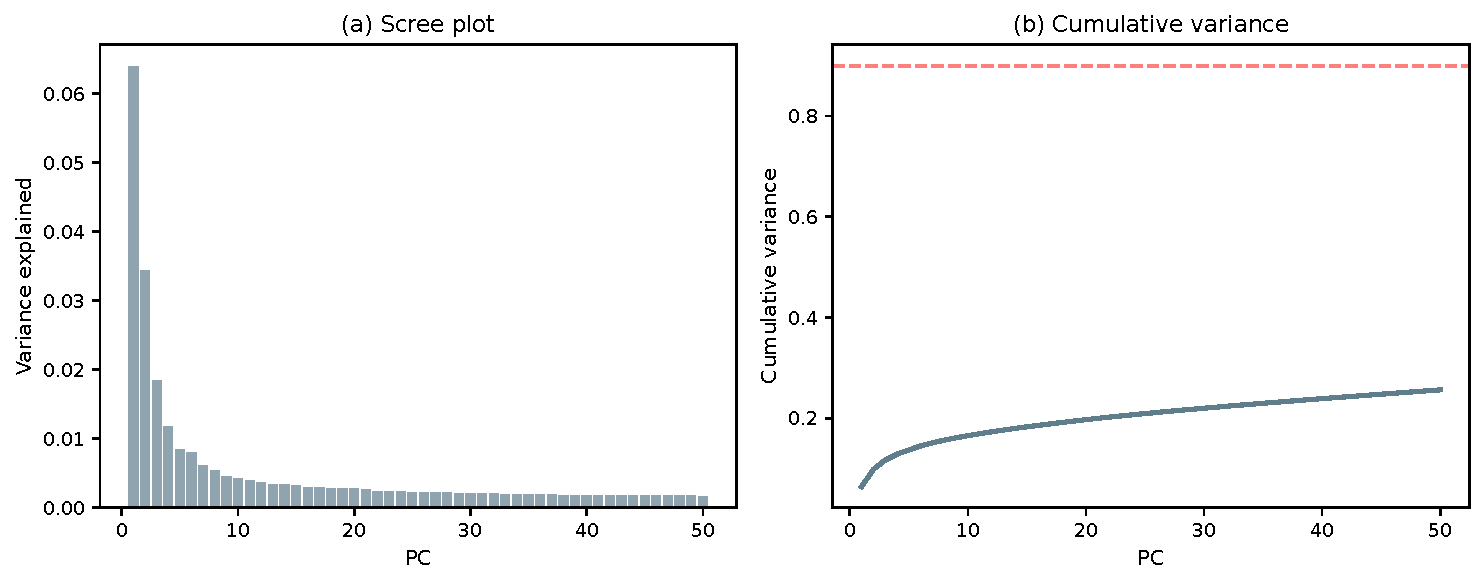
\includegraphics[width=\textwidth]{figS4_pca.pdf}
\caption{\textbf{Figure S4: PCA variance explained.} Scree plot and cumulative variance for the 50-component PCA used as input to the diffusion map and dispersion analyses.}
\label{fig:S4}
\end{figure}

\begin{figure}[H]
\centering
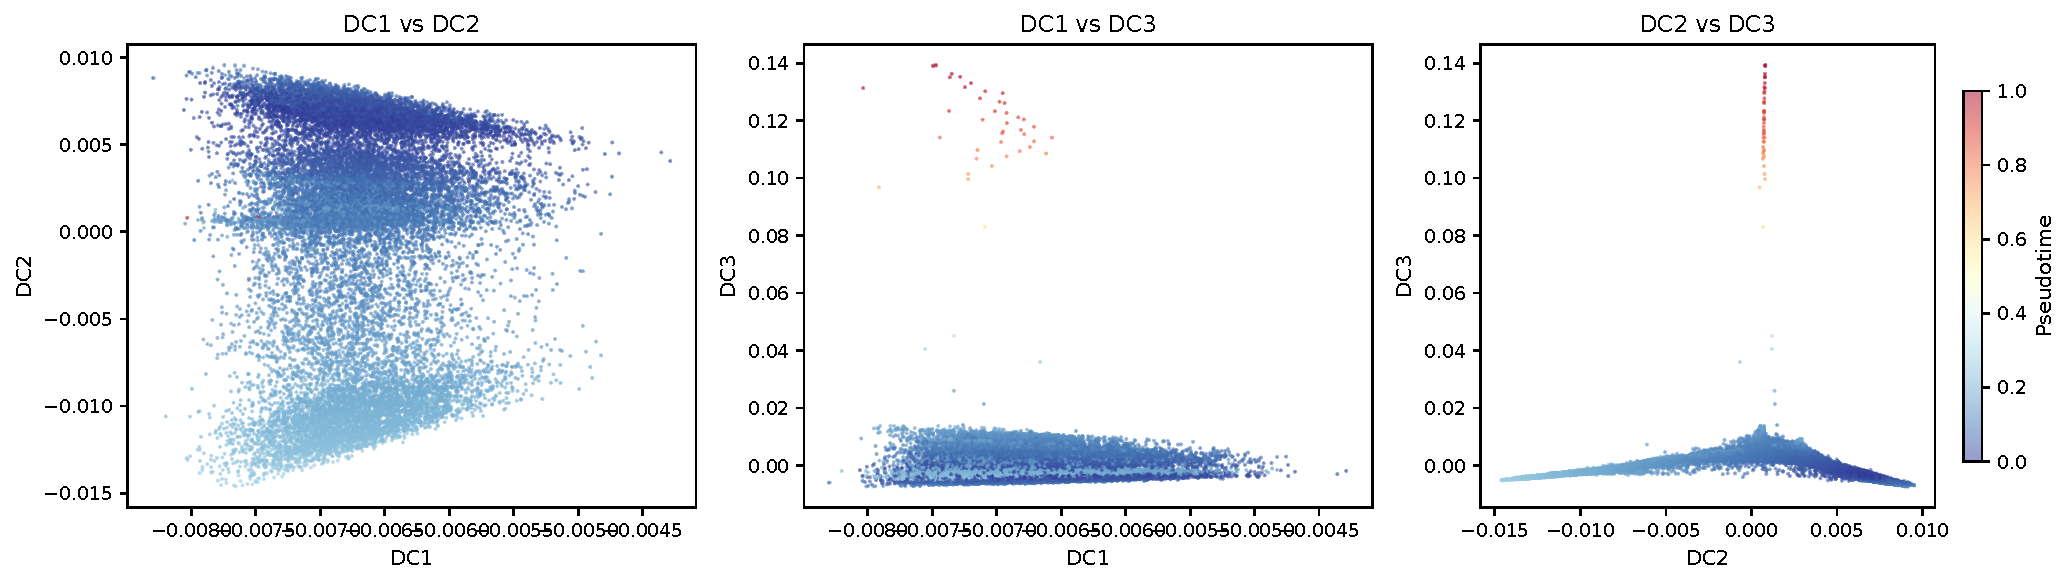
\includegraphics[width=\textwidth]{figS5_diffmap.pdf}
\caption{\textbf{Figure S5: Diffusion map components.} First three diffusion components colored by condition, cell type, and pseudotime, showing the manifold structure underlying the pseudotime ordering.}
\label{fig:S5}
\end{figure}

\begin{figure}[H]
\centering
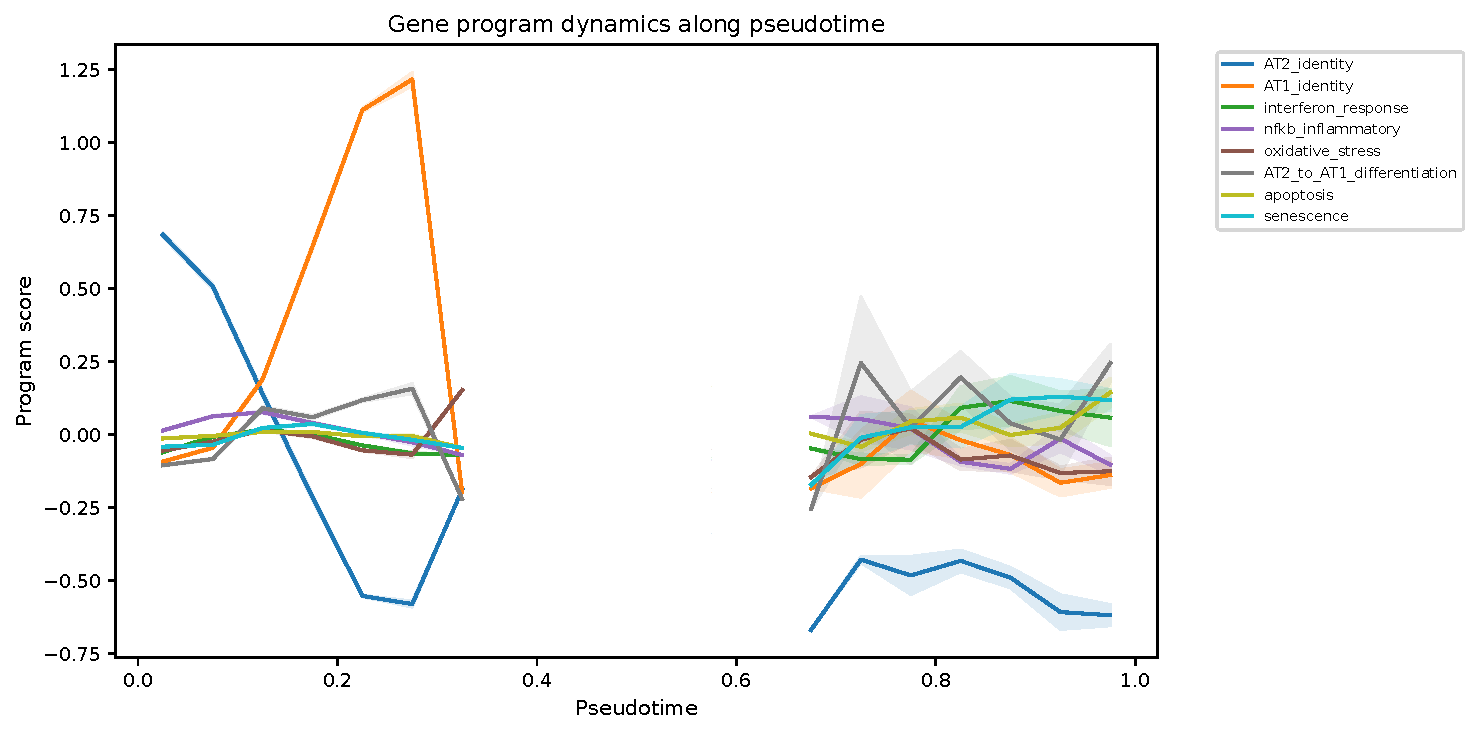
\includegraphics[width=\textwidth]{figS6_program_dynamics.pdf}
\caption{\textbf{Figure S6: Gene-program dynamics along pseudotime.} Mean program scores across 20 equal-width pseudotime bins for all eight gene programs, stratified by condition. Homeostatic programs (AT2, AT1 identity) decline with pseudotime; injury programs rise in the upper half.}
\label{fig:S6}
\end{figure}

\begin{figure}[H]
\centering
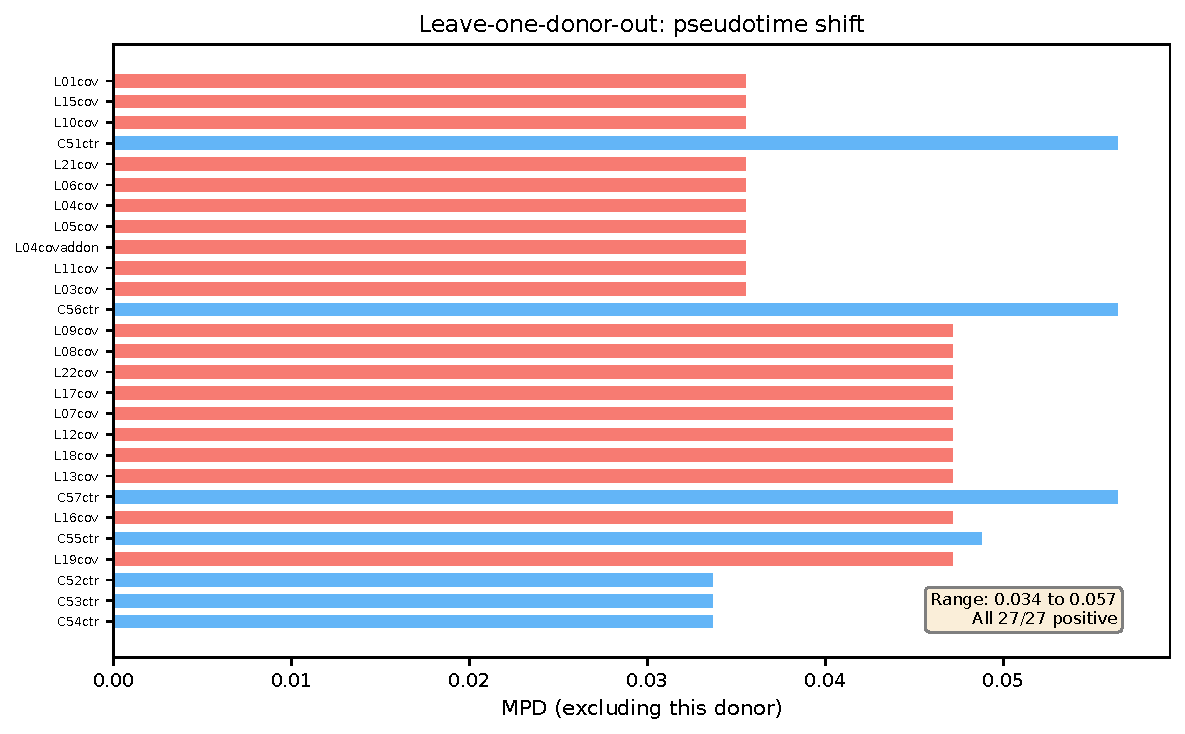
\includegraphics[width=\textwidth]{figS9_lodo.pdf}
\caption{\textbf{Figure S9: Leave-one-donor-out analysis.} Median pseudotime difference for each of 27 iterations, confirming that no single donor drives the pseudotime shift (range 0.028--0.202; all positive).}
\label{fig:S9}
\end{figure}

\begin{figure}[H]
\centering
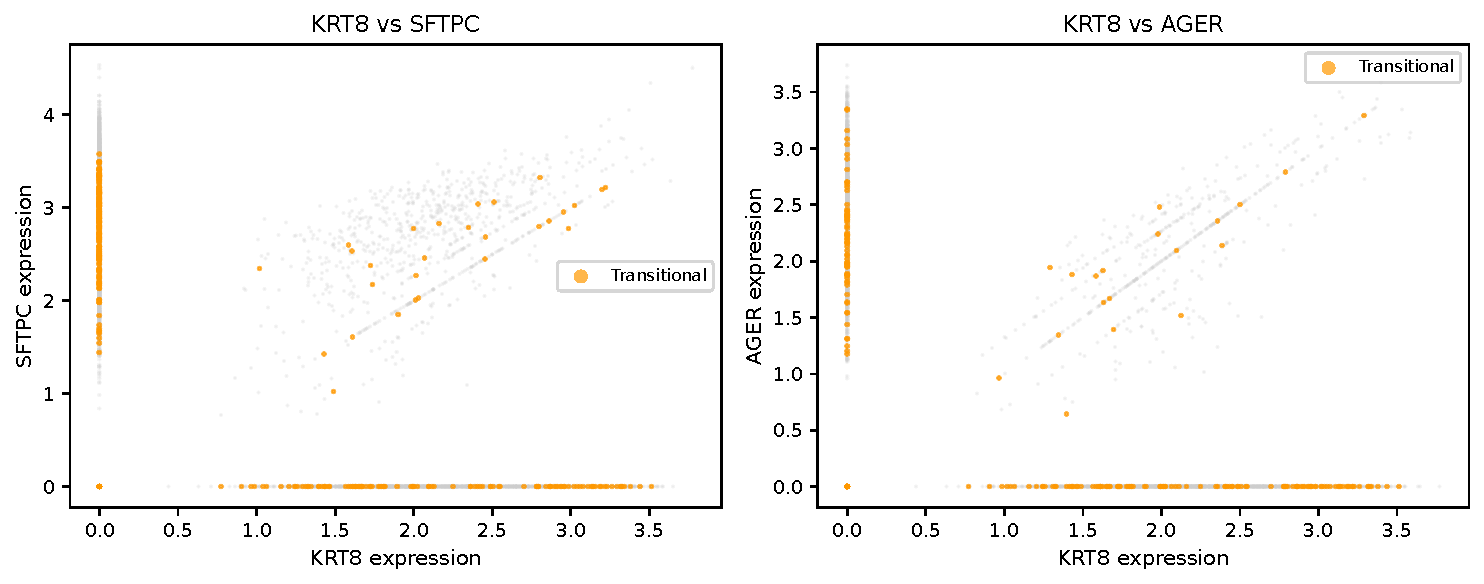
\includegraphics[width=\textwidth]{figS10_transitional.pdf}
\caption{\textbf{Figure S10: Transitional cell characterization.} Extended marker analysis and pseudotime distribution for the ECM-high transitional compartment.}
\label{fig:S10}
\end{figure}

\begin{figure}[H]
\centering
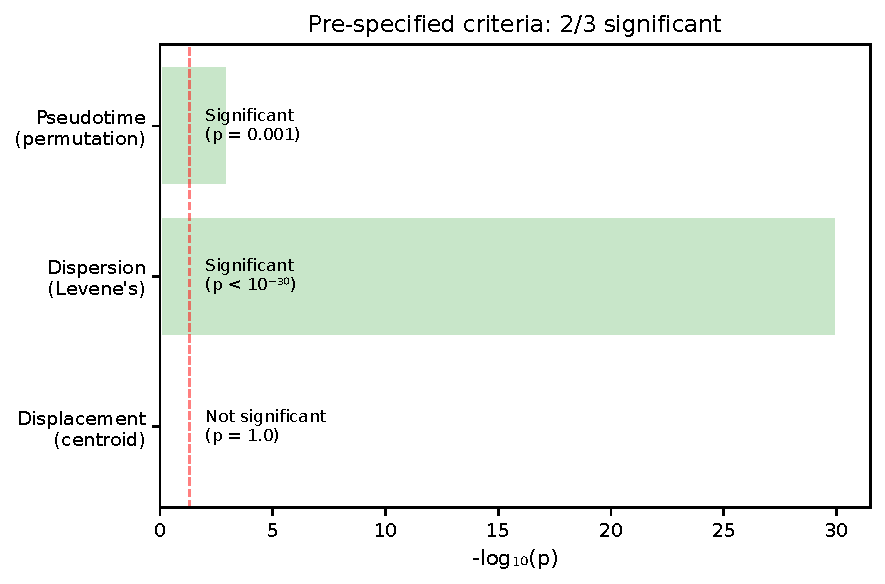
\includegraphics[width=\textwidth]{figS11_composite.pdf}
\caption{\textbf{Figure S11: Injury composite score.} Distribution of the six-program injury composite score by condition in both primary and replication cohorts.}
\label{fig:S11}
\end{figure}

\begin{figure}[H]
\centering
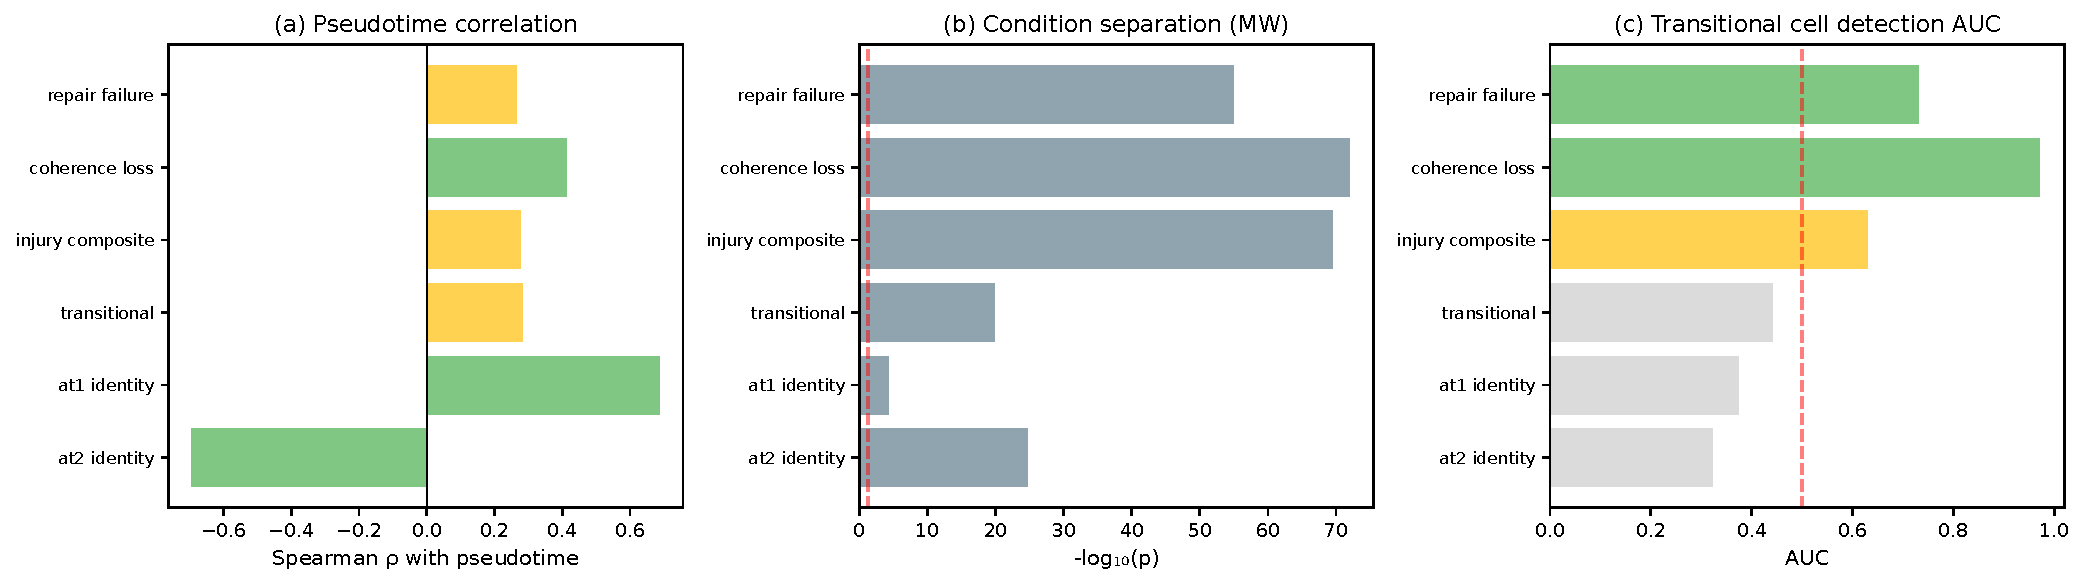
\includegraphics[width=\textwidth]{figS12_state_scores.pdf}
\caption{\textbf{Figure S12: Portable state scores.} Distributions of all six continuous state scores (AT2 identity, AT1 identity, transitional, injury composite, coherence loss, repair failure) by condition, with benchmark statistics.}
\label{fig:S12}
\end{figure}

\begin{figure}[H]
\centering
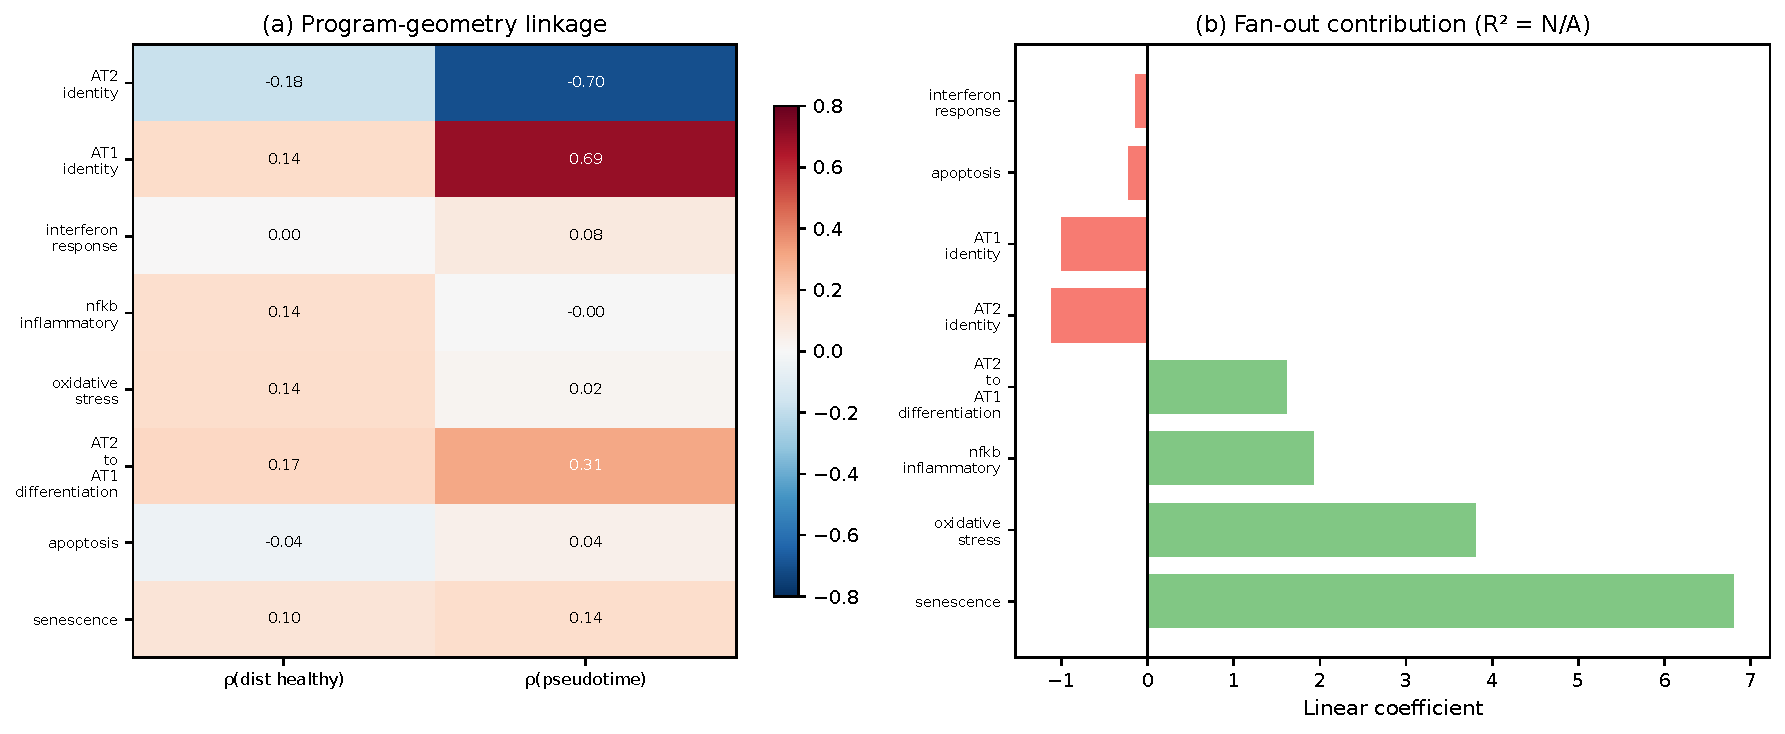
\includegraphics[width=\textwidth]{figS13_mechanism.pdf}
\caption{\textbf{Figure S13: Mechanistic decomposition.} \textbf{(a)} Program-geometry linkage: Spearman correlations of each program with distance-to-healthy-centroid and pseudotime. \textbf{(b)} Fan-out regression coefficients ($R^2 = 0.115$). \textbf{(c)} Repair-stall analysis: differentiation/apoptosis ratio across pseudotime bins by condition.}
\label{fig:S13}
\end{figure}

\end{document}
